\documentclass{libs/XJTLU_format}
% Inserting the preamble file with the packages
%%%%%%%%%%%%%%%%%%%%%%%%%%%%%%%%%%%%%%%%%%%%%%%%%%%%%%%%%%%%%%%%%%%%%
%% This file contains the packages that can be used in the beamer. %%
%%%%%%%%%%%%%%%%%%%%%%%%%%%%%%%%%%%%%%%%%%%%%%%%%%%%%%%%%%%%%%%%%%%%%
% Package to fonts family
\usepackage[T1]{fontenc}
% Package to accentuation
\usepackage[utf8]{inputenc}
% Package to Figures
\usepackage{graphicx}
% Package to the colors
\usepackage{color}
% Package to the colors
\usepackage{xcolor}
% Packages to math symbols and expressions
\usepackage{amsfonts, amssymb, amsmath}
% Package to multiple lines and columns in table
\usepackage{multirow, array} 
% Package to create pseudo-code
% For more detail of this package: http://linorg.usp.br/CTAN/macros/latex/contrib/algorithm2e/doc/algorithm2e.pdf
\usepackage{algorithm2e}
% Package to insert code
\usepackage{listings} 
\usepackage{keyval}
% Package to justify text
\usepackage[document]{ragged2e}
% Package to manage the bibliography
\usepackage[backend=biber, style=numeric, sorting=none]{biblatex}
% Package to facilities quotations
\usepackage{csquotes}
% Package to use multicols
\usepackage{multicol}
\usepackage{transparent}

% Inserting the references file
\bibliography{references.bib}
\uselanguage{French}
\languagepath{French}

% Title
\title[Sécurisation de la migration des machines virtuelles]{\huge\textbf{Sécurisation de la migration des machines virtuelles}}
% Subtitle
% Author of the presentation
\author{Salim NEDJAM}
\institute[]{
    % Department Name
    \department{
        Réferent: Pierre SENS \hspace{1.5cm} Encadrant: Antoine BLIN
    }
    \newline
    % University name
    \department{
        
\includegraphics[scale=0.2]{images/logo_sorbonne.png}
        \hspace{2cm}
        
\includegraphics[scale=0.1]{images/logo_gandi.png}
    }}
% date of the presentation
\date{\today}

%%%%%%%%%%%%%%%%%%%%%%%%%%%%%%%%%%%%%%%%%%%%%%%%%%%%%%%%%%%%%%%%%%%%%%%%%%%%%%%%%%
%% Start Document of the Presentation                                           %%               
%%%%%%%%%%%%%%%%%%%%%%%%%%%%%%%%%%%%%%%%%%%%%%%%%%%%%%%%%%%%%%%%%%%%%%%%%%%%%%%%%%
\begin{document}
% insert the code style
%%%%%%%%%%%%%%%%%%%%%%%%%%%%%%%%%%%%%%%%%%%%%%%%%%%%%%%%%%%%%%%%%%%%%%%%%%%%%%%%%%%
%% This file contains the style of the codes show in slides.                     %%
%% The package used is listings, but it possible to used others.                 %%
%%%%%%%%%%%%%%%%%%%%%%%%%%%%%%%%%%%%%%%%%%%%%%%%%%%%%%%%%%%%%%%%%%%%%%%%%%%%%%%%%%%

% color used in the code style
\definecolor{codegreen}{rgb}{0,0.6,0}
\definecolor{codegray}{rgb}{0.5,0.5,0.5}
\definecolor{codepurple}{rgb}{0.58,0,0.82}
\definecolor{codebackground}{rgb}{0.95,0.95,0.92}

% style of the code!
\lstdefinestyle{codestyle}{
    backgroundcolor=\color{codebackground},   
    commentstyle=\color{codegreen},
    keywordstyle=\color{magenta},
    numberstyle=\tiny\color{codegray},
    stringstyle=\color{codepurple},
    basicstyle=\ttfamily\footnotesize,
    frame=single,
    breakatwhitespace=false,         
    breaklines=true,                 
    captionpos=b,                    
    keepspaces=true,                 
    numbers=left,                    
    numbersep=5pt,                  
    showspaces=false,                
    showstringspaces=false,
    showtabs=false,                  
    tabsize=2,
    title=\lstname 
}

\lstset{style=codestyle}


%% ---------------------------------------------------------------------------
% First frame (with tile, subtitle, ...)
\begin{frame}[noframenumbering]{}
    \maketitle
\end{frame}

%\begin{frame}[noframenumbering]{}
%\tableofcontents[hideallsubsections]
%\end{frame}
%% ---------------------------------------------------------------------------
% This presentation is separated by sections and subsections
\section{Contexte général}
\begin{frame}{Virtualisation}
    \only<1>{
        \begin{figure}
        \centering
        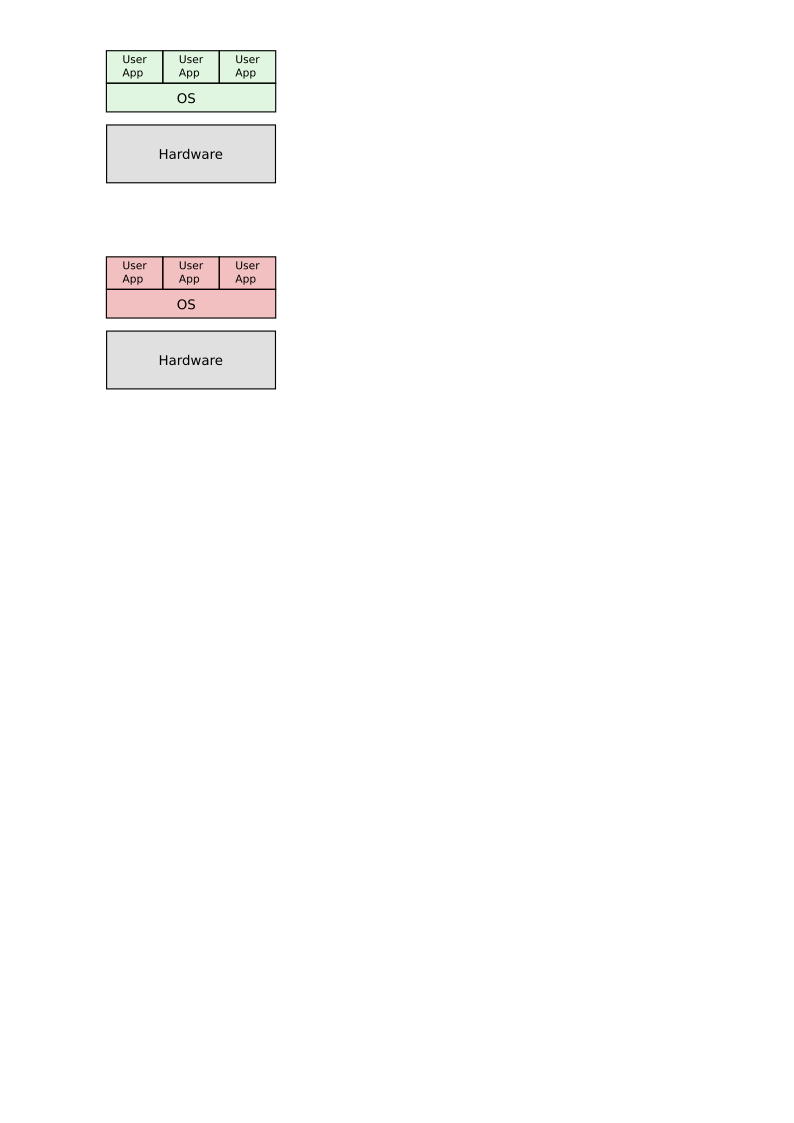
\includegraphics[scale=0.5]{images/virt1.png}
        \end{figure}
    }
    \only<2>{
        \begin{figure}
        \centering
        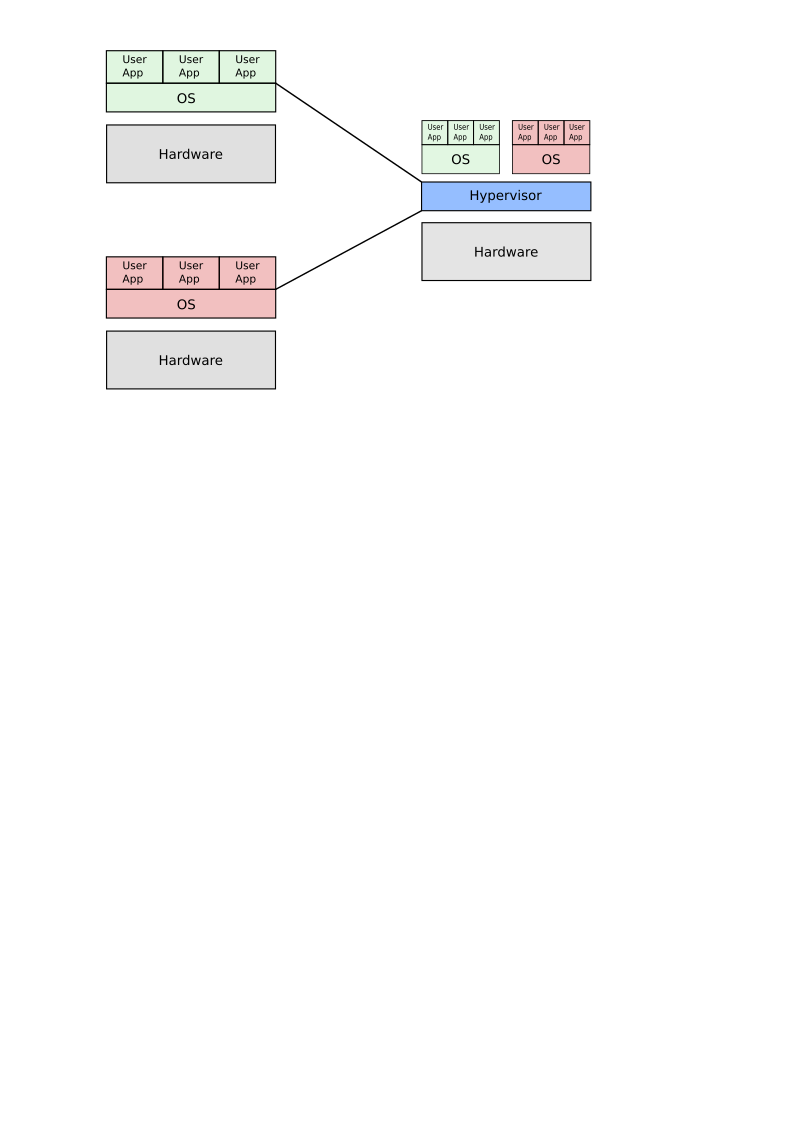
\includegraphics[scale=0.5]{images/virt2.png}
        \end{figure}
    }
\end{frame}
\begin{frame}{Sécurisation des migrations de VM}
    \only<1>{
        Avantages:
        \begin{itemize}
            \item La consolidation des serveurs.
            \item Équilibrage de la charge.
            \item Maintenance matérielle sans temps d'arrêt.
        \end{itemize}
    }
    \only<2> {
        Problèmes:
        \begin{itemize}
            \item Sécuriser les VMs pendant la migration.
            \item Sécuriser l'intégrité des données des VMs.
        \end{itemize}
    }
    
\end{frame}

\section{Contexte technique}
\begin{frame}{Migration de VM: LAN}
    \begin{figure}
        \centering
        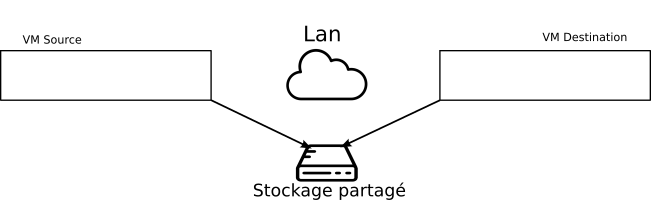
\includegraphics[scale=0.5]{images/lan.png}
    \end{figure}
    \begin{enumerate}
        \item Les VMs sont sur le même réseau local.
        \item Disque partagé (NFS/SAN).
        \item Pas de transfert des données du disque.
    \end{enumerate}
\end{frame}

\begin{frame}{Migration de VM: WAN}
    \begin{figure}
        \centering
        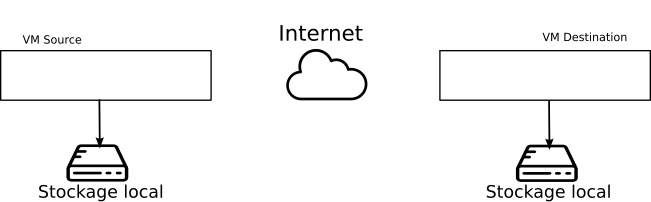
\includegraphics[scale=0.5]{images/wan.png}
    \end{figure}
    \begin{enumerate}
        \item Les VMs sont sur des machines distantes.
        \item Pas de disque partagé (NFS/SAN).
        \item Le transfert des données du disque est obligatoire.
    \end{enumerate}
\end{frame}

\begin{frame}{Migration à froid}
    \only<1>{
        \begin{figure}
        \centering
        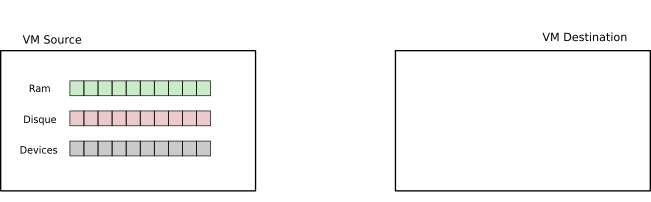
\includegraphics[scale=0.5]{images/froid1.png}
        \end{figure}
    }
    \only<2>{
        \begin{figure}
        \centering
        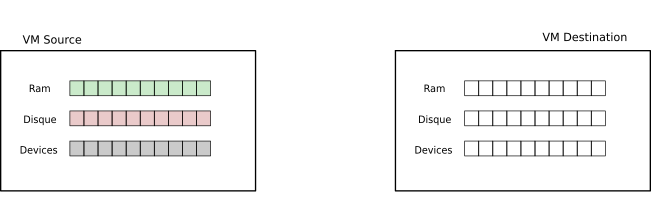
\includegraphics[scale=0.5]{images/froid2.png}
        \end{figure}
    }
    \only<3>{
        \begin{figure}
        \centering
        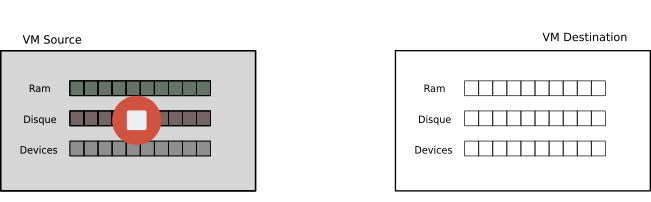
\includegraphics[scale=0.5]{images/froid3.png}
        \end{figure}
    }
    \only<4-5>{
        \begin{figure}
        \centering
        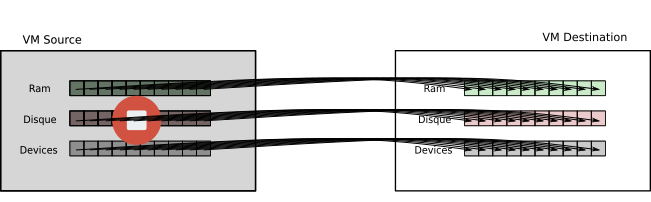
\includegraphics[scale=0.5]{images/froid4.png}
        \end{figure}
    }
    \only<1-4>{
        \begin{enumerate}
            \item<2-> Allocation d'une VM de même caractéristiques.
            \item<3-> Stoper la machine.
            \item<4-> Transfert de tous les périphériques.
        \end{enumerate}
    }
    \only<5>{
        \color{red} Temps d'arrêt = Temps total de migration.   
    }
\end{frame}

\begin{frame}{Migration à chaud: pre-copie}
        \only<1>{
            \begin{figure}
            \centering
            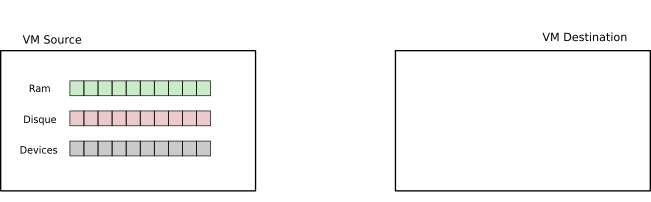
\includegraphics[scale=0.5]{images/pre1.png}
            \end{figure}
        }
        \only<2>{
            \begin{figure}
            \centering
            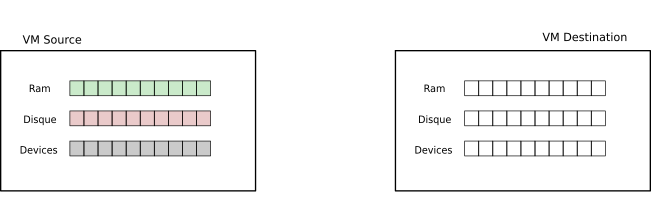
\includegraphics[scale=0.5]{images/pre2.png}
            \end{figure}
        }
        \only<3>{
            \begin{figure}
            \centering
            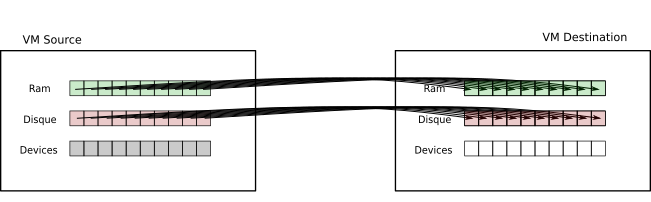
\includegraphics[scale=0.5]{images/pre3.png}
            \end{figure}
        }
        \only<4>{
            \begin{figure}
            \centering
            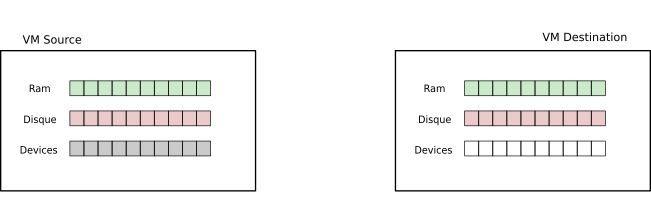
\includegraphics[scale=0.5]{images/pre4.png}
            \end{figure}
        }
        \only<5>{
            \begin{figure}
            \centering
            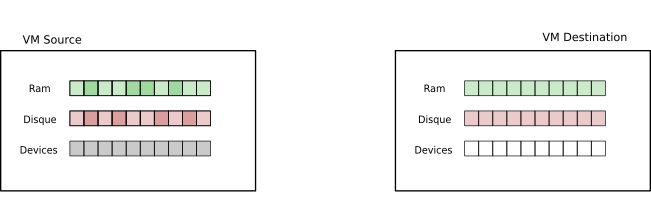
\includegraphics[scale=0.5]{images/pre5.png}
            \end{figure}
        }
        \only<6>{
            \begin{figure}
            \centering
            
\includegraphics[scale=0.5]{images/pre6.png}
            \end{figure}
        }
        \only<7>{
            \begin{figure}
            \centering
            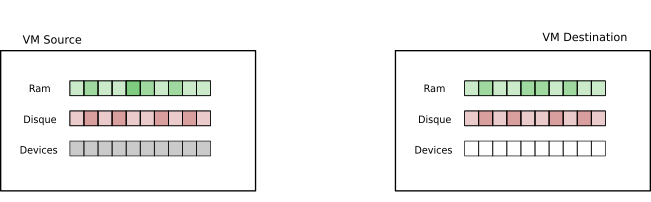
\includegraphics[scale=0.5]{images/pre7.png}
            \end{figure}
        }
        \only<8>{
            \begin{figure}
            \centering
            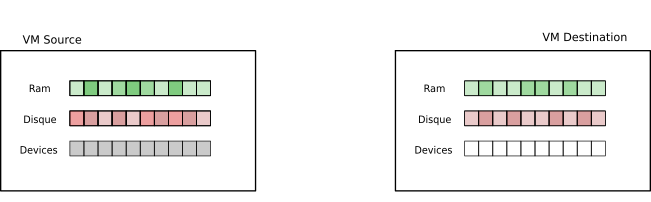
\includegraphics[scale=0.5]{images/pre8.png}
            \end{figure}
        }
        \only<9>{
            \begin{figure}
            \centering
            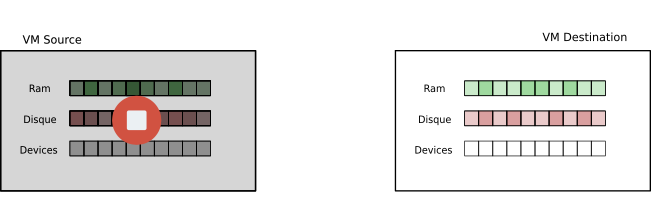
\includegraphics[scale=0.5]{images/pre9.png}
            \end{figure}
        }
        \only<10>{
            \begin{figure}
            \centering
            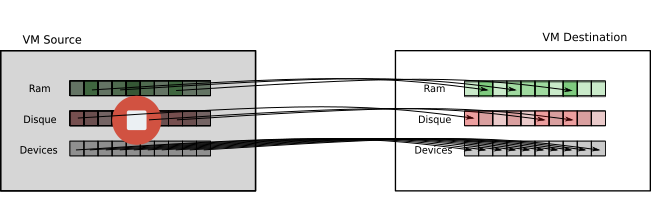
\includegraphics[scale=0.5]{images/pre10.png}
            \end{figure}
        }

        \only<2-10>{
            \begin{enumerate}
                \item<2-> Allocation d'une VM de même caractéristiques.
                \item<3-> Copie des périphériques itératifs.
                    \begin{enumerate}
                        \item<4-> Première itération.
                        \item<5-> Génération des pages dirty \only<6->{-> Copie des pages dirty}
                        \item<7-> Tester les critères de convergences.
                    \end{enumerate}
                \item<9-> Stoper la machine.
                \item<10> Copie de tous les périphériques.
            \end{enumerate}
        }
        \only<11>{
            \color{green} Temps d'arrêt = Temps de la dernière itération.
        }
\end{frame}

\begin{frame}{Migration à chaud: post-copie}
    \only<1>{
        \begin{figure}
        \centering
        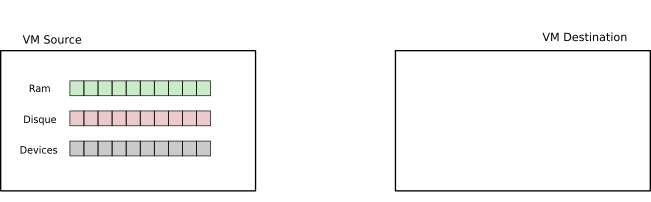
\includegraphics[scale=0.5]{images/post1.png}
        \end{figure}
    }
    \only<2>{
        \begin{figure}
        \centering
        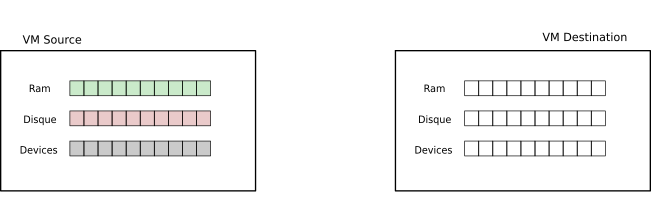
\includegraphics[scale=0.5]{images/post2.png}
        \end{figure}
    }
    \only<3>{
        \begin{figure}
        \centering
        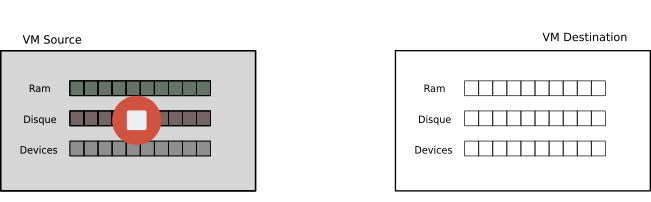
\includegraphics[scale=0.5]{images/post3.png}
        \end{figure}
    }
    \only<4>{
        \begin{figure}
        \centering
        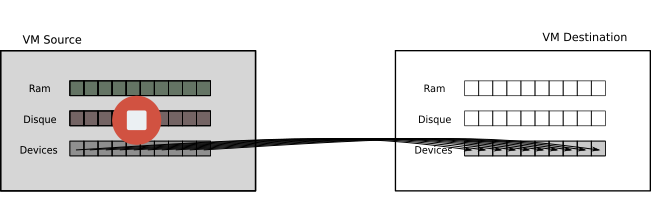
\includegraphics[scale=0.5]{images/post4.png}
        \end{figure}
    }
    \only<5-10>{
        \begin{figure}
        \centering
        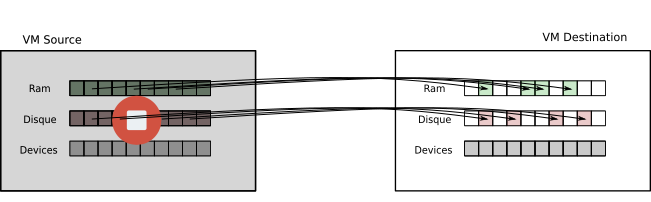
\includegraphics[scale=0.5]{images/post5.png}
        \end{figure}
    }
    \only<2-9>{
        \begin{enumerate}
            \item<2-> Allocation d'une VM de même caractéristiques.
            \item<3-> Stoper la machine.
            \item<4-> Transfert des structures de données essentielles.
            \item<5-> Transfert des pages mémoire: 
            \begin{enumerate}
                \item<6-> Demand-paging
                \item<7-> Active-push
                \item<8-> Pre-paging
                \item<9-> Dynamic self balooning
            \end{enumerate}
        \end{enumerate}   
    }
    \only<10>{
            \begin{itemize}
                \item \color{green} Temps d'arrêt = Transfert des structures de données essentielles.
                \item \color{red} Ralentissement de la VM destination.
                \item \color{red} Risque de perte des données. 
            \end{itemize}  
        }
\end{frame}



\begin{frame}{Calcul d'empreinte}
    
    \only<1>{
        \begin{figure}
        \centering
        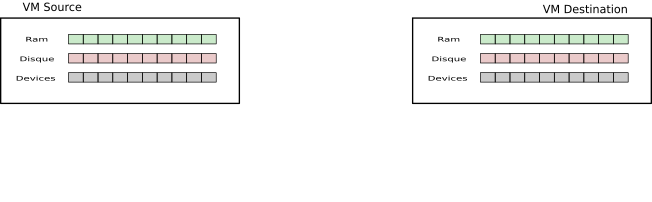
\includegraphics[scale=0.5]{images/hash0.png}
        \end{figure}
    }
    \only<2>{
        \begin{figure}
        \centering
        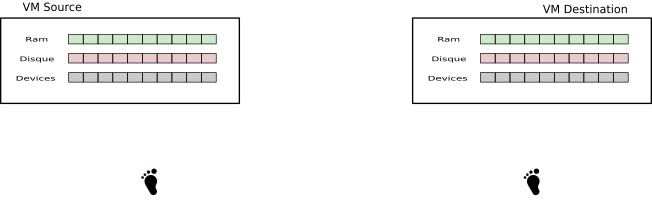
\includegraphics[scale=0.5]{images/hash1.png}
        \end{figure}
    }
    \only<3>{
        \begin{figure}
        \centering
        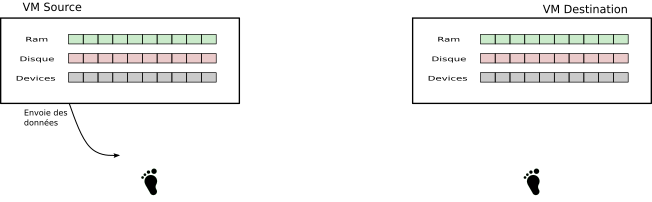
\includegraphics[scale=0.5]{images/hash2.png}
        \end{figure}
    }
    \only<4>{
        \begin{figure}
        \centering
        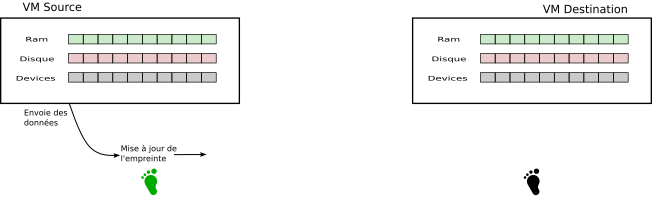
\includegraphics[scale=0.5]{images/hash3.png}
        \end{figure}
    }
    \only<5>{
        \begin{figure}
        \centering
        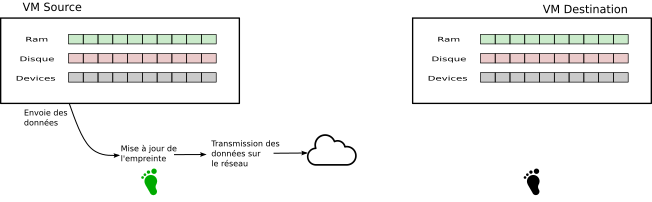
\includegraphics[scale=0.5]{images/hash4.png}
        \end{figure}
    }
    \only<6>{
        \begin{figure}
        \centering
        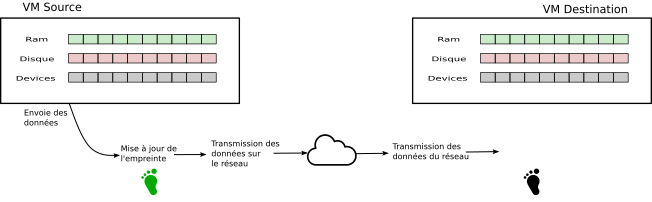
\includegraphics[scale=0.5]{images/hash5.png}
        \end{figure}
    }
    \only<7->{
        \begin{figure}
        \centering
        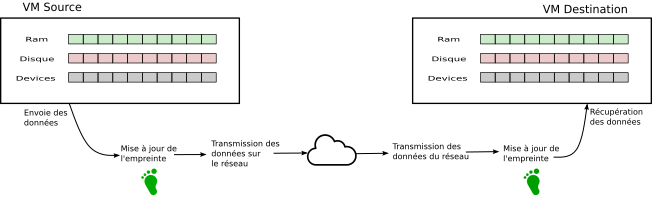
\includegraphics[scale=0.5]{images/hash6.png}
        \end{figure}
    }
    \only<1-2>{
        \begin{description}
            \item<1-2>[Problématique] S'assurer de l'intégrité des données.
            \bigskip 
            \item<2>[Solution] Génération de l'empreinte de chaque VM.
        \end{description}
    }
    \only<3-8>{
        \begin{enumerate}
            \item<3-8> Envoie des données de la VM.
            \item<4-8> Calcul de la nouvelle empreinte de la VM source.
            \item<5-8> Transmission des données de la VM sur le réseau.
            \item<6-8> Réception des données de la VM du le réseau.
            \item<7-8> Calcul de la nouvelle empreinte de la VM destination.
            \item<8> Mise à jour des données de la VM.
        \end{enumerate}

    }

    
\end{frame}


\section{Contribution}
\begin{frame}{Scénario 1}
    \begin{figure}
        \centering
        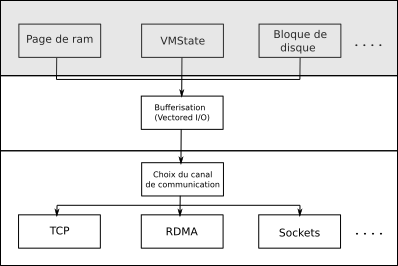
\includegraphics[scale=0.5]{images/idea2.png}
    \end{figure}
    Avantages:
        \begin{enumerate}
            \item Connaissance du type de données envoyées.
            \item Envoyer que les données importantes pour l'empreinte.
        \end{enumerate}
        Inconvénients:
        \begin{enumerate}
            \item Non générique.
            \item Rajout du code dans tout les périphériques
        \end{enumerate}
\end{frame}

\begin{frame}{Scénario 2}
    \begin{figure}
        \centering
        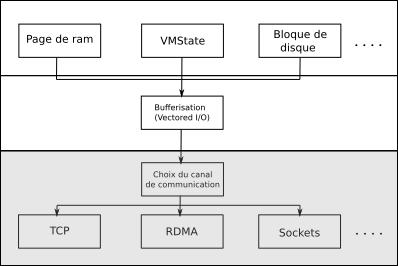
\includegraphics[scale=0.5]{images/idea4.png}
    \end{figure}
    Inconvénient:
        \begin{enumerate}
            \item Modifier le code de tout les protocoles réseau.
            \item Pas de connaissance du type de données envoyées.
        \end{enumerate}
\end{frame}

\begin{frame}{Scénario 3}
    \begin{figure}
        \centering
        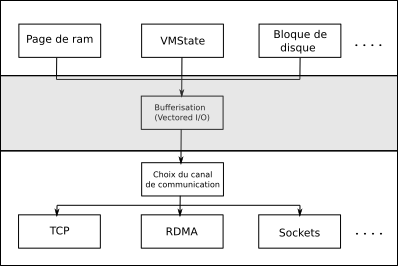
\includegraphics[scale=0.5]{images/idea3.png}
    \end{figure}
    Avantages:
        \begin{enumerate}
            \item Générique.
            \item Facile, peu de code à rajouter.
        \end{enumerate}
    Inconvénients:
        \begin{enumerate}
            \item Connaissance limitée du type de données envoyées.
            \item Headers de section sont inclut dans le calcul de l'empreinte.
        \end{enumerate}
\end{frame}

\section{Evaluation}
\begin{frame}{Métriques de performances}
    \begin{description}
        \item[Temps de migration] Temps entre le début de la migration et le moment où l'hôte source peut être désactivé.
        \item[Temps d'arrêt (Downtime)] Phase indisponibilité du service perceptible par l'utilisateur.
    \end{description}
\end{frame}

\begin{frame}{Benchmark: Taille de la mémoire}
    \only<1-2>{
        Varier la taille mémoire de la VM.
    }
    \only<2>{
        \newline
        \bigskip
        Configurations possible: 512 Mo, 1 Go, 2 Go, 4 Go et 8 Go.
    }
    \only<3>{
        \begin{figure}[H]
            \begin{minipage}{0.48\textwidth}
                \centering
                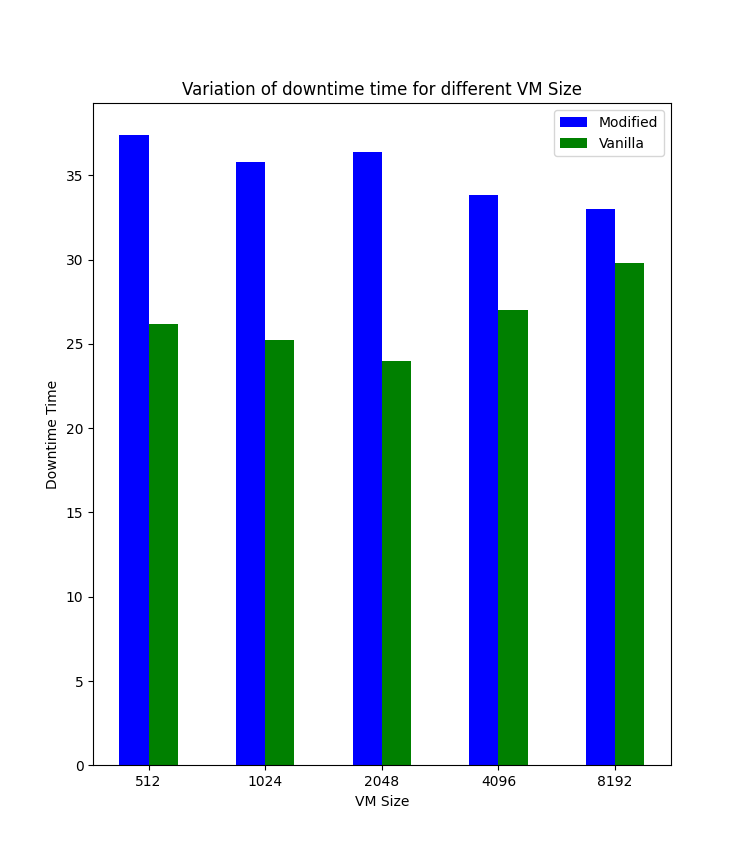
\includegraphics[width=1\linewidth]{images/down_vmsize.png}
            \end{minipage}\hfill
            \begin{minipage}{0.48\textwidth}
                \centering
                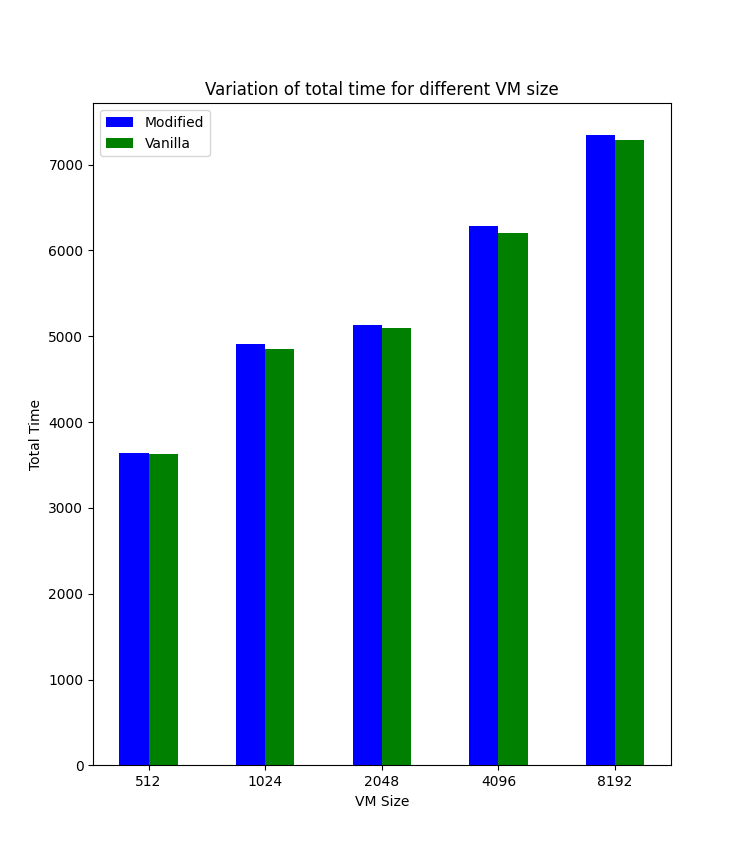
\includegraphics[width=1\linewidth]{images/total_vmsize.png}
            \end{minipage}
        \end{figure}
    }
\end{frame}

\begin{frame}{Benchmark: Vitesse d'écriture}
    \only<1-2>{
        Création d'un processus dont le but est de salir la mémoire.
    }
    \only<2>{
        \newline
        \bigskip
        Le but est de forcer plusieurs itération de la migration.
    }
    \only<3>{
        \begin{figure}[H]
            \begin{minipage}{0.48\textwidth}
                \centering
                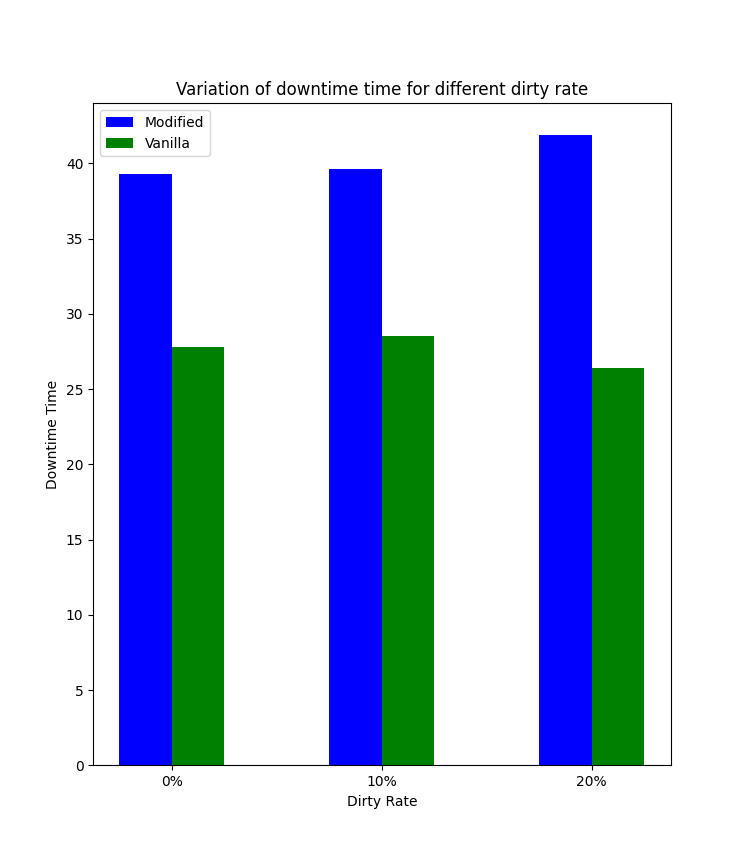
\includegraphics[width=1\linewidth]{images/down_rate.png}
            \end{minipage}\hfill
            \begin{minipage}{0.48\textwidth}
                \centering
                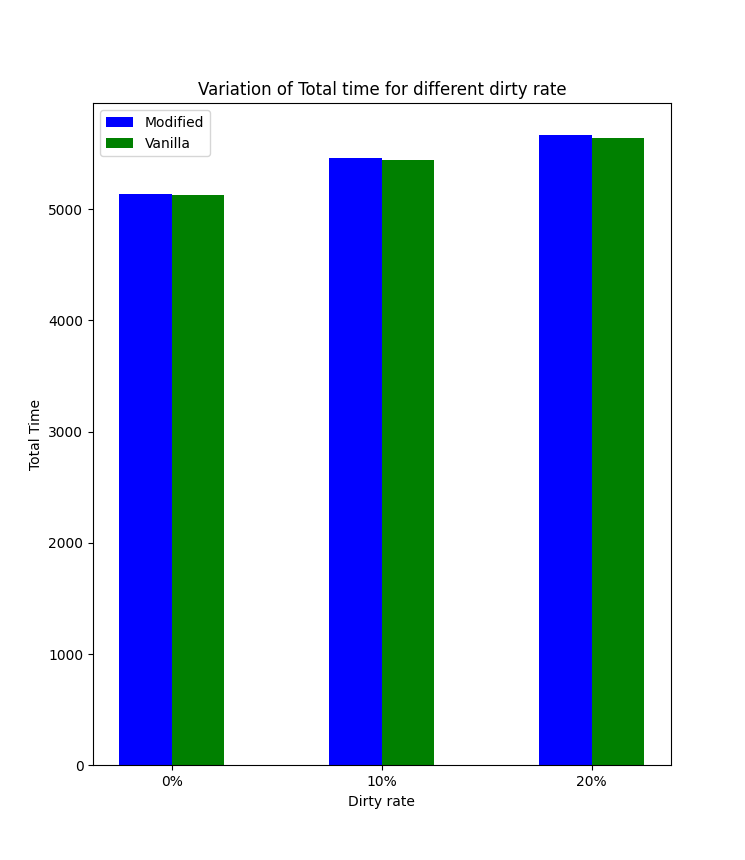
\includegraphics[width=1\linewidth]{images/total_rate.png}
            \end{minipage}
        \end{figure}
    }

\end{frame}

\begin{frame}{Benchmark: Résultats}
    Overhead de 10ms pour le downtime.
    \newline
    \bigskip
    Overhead en temps total est de l'ordre de moins de 1\%.

\end{frame}

\section{Conclusion}
\begin{frame}{Conclusion et Proposition d'optimisation}
    Conclusion
    \begin{enumerate}
        \item Génération d'une empreinte de VM.
        \item Migration en direct avec/sans disque partagé.
        \item Analyse du code de migration QEMU.
        \item Analyse du flux réseau.
        \item Problématique du mappage direct des données.
    \end{enumerate}
    Proposition d'optimisation
    \begin{enumerate}
        \item Calcul du hash dans un thread différent (multi-threading).
        \item Hashage intelligent des pages dirty.
        \item Hashage intelligent des pages vides.
        \item Hashage des données plus fin.
    \end{enumerate}

\end{frame}
\end{document}